\subsection{Bianisotropic media considered in \cite{alottocodecasa}}
Another instance of a relevant bianisotropic media was considered in 
\cite{alottocodecasa}, where the authors consider a rectangular waveguide, 
half of which is empty and the other half is filled with a lossless bianisotropic material characterized by 

\begin{equation} \label{constitutive_alotto_P}
P = \varepsilon_0c_0 I_3,
\end{equation}

\begin{equation} \label{constitutive_alotto_Q}
Q = \frac{1}{\mu_0c_0} I_3, 
\end{equation}

\begin{equation} \label{constitutive_alotto_LM}
L = M = j\kappa_0 A ,
\end{equation}
where $A$ is the matrix given by

\begin{equation} \label{constitutive_alotto_LM}
A= 
\begin{bmatrix}
1 & 1 & 0 \\
1 & 1 & 0 \\
0 & 0 & 1 
\end{bmatrix},
\end{equation}
where $\kappa_0$ is a positive real number.

The hypotheses H5 and H6 are trivially valid with $C_{PS} = \varepsilon_0c_0$ and
$C_{QS} = \frac{1}{\mu_0c_0}$.
Further, $L^*L = M^*M =  \kappa_0^2A^2$ whose eigenvalues are 0, $\kappa_0^2$ and $4\kappa_0^2$.
Therefore by equations \eqref{equation_for_CL} and \eqref{equation_for_CM} we get $C_L = C_M = 2\kappa_0$.
The condition in hypothesis H7 then becomes 
$C_{QS} - \frac{C_L C_M}{C_{PS}} = \frac{1}{\mu_0c_0} - \frac{4\kappa_0^2}{\varepsilon_0c_0} > 0$, 
which gives the following limit on $\kappa_0$.

\begin{equation} \label{eq:uniqueness_cond_alotto_codecasa}
\kappa_0 < \frac{1}{2}\sqrt{\frac{\varepsilon_0}{\mu_0}} = 1.327 \, 10^{-3}   \text{ mho }
\end{equation}

The hypotheses H1 to H4 can be studied using the alternative form of constitutive relations
which is characterized by the following matrices \cite{noiregolarita}.

\begin{equation}
\kappa =\frac{1}{\varepsilon_0}I_3
\end{equation}

\begin{equation}
\nu =\frac{1}{\mu_0}I_3 + \frac{\kappa_0^2}{\varepsilon_0}A^2
\end{equation}

\begin{equation}
\chi = -\gamma = \frac{-j\kappa_0}{\varepsilon_0}A
\end{equation}

The determinants of $\kappa$ and $\nu$ can be readily calculated and by using equations
\eqref{equation_for_C_kd} and \eqref{equation_for_C_nud} we get $C_{\kappa,d}$ and $C_{\nu,d}$.

\begin{equation}
C_{\kappa,d} = \frac{1}{\varepsilon_0^3}
\end{equation}

\begin{equation}
C_{\nu,d} =  \frac{(\varepsilon_0+\mu_0\kappa_0^2)(\varepsilon_0+4\mu_0\kappa_0^2)}{\mu_0^3\varepsilon_0^2}
\end{equation}

$C_{\kappa,s}$ and $C_{\nu,s}$ can be directly obtained from their definitions.

\begin{equation}
C_{\kappa,s} = \frac{2}{\varepsilon_0}
\end{equation}

\begin{equation}
C_{\nu,s} = \frac{2\varepsilon_0 + 8\mu_0\kappa_0^2}{\mu_0\varepsilon_0}
\end{equation}

By simple application of the definition
\begin{equation}
C_{\kappa,r} = \varepsilon_0 ,
\end{equation}
and by equation \eqref{equation_for_C_nur}  $C_{\nu,r}$ evaluates to the reciprocal of the largest 
eigenvalue of the real matrix $\nu$ which is given by
\begin{equation}
C_{\nu,r} =  \frac{\mu_0\varepsilon_0}{\varepsilon_0 + 4 \mu_0\kappa_0^2}.
\end{equation}

The equations  \eqref{equation_for_C_chis} and \eqref{equation_for_C_gammas} give 

\begin{equation}
C_{\chi,s} = C_{\gamma,s}= = \frac{4\kappa_0}{\varepsilon_0}.
\end{equation}

The existence of the above constants verifies H1 -H3 and we can use them to 
calculate $K_u$ to verify H4.
It can be verified that $K_u$ is less than one when $\kappa_0 \leq 2.72 \, 10^{-4}$ mho,
which is stricter than the limit obtained from equation \eqref{eq:uniqueness_cond_alotto_codecasa}.

Finally let us give some numerical solutions for this problem, which can be used as benchmarks for other 
approaches.
The cross section of the waveguide is such that it is 2 cm along the x axis and  1 cm along the y axis, and 
the length of the waveguide is 2 cm, half of which is filled with the bianisotropic medium  characterized by 
$\kappa_0 = 2.7 \, 10^{-3}$.
The origin is taken on the corner of the open face of the waveguide on the empty side.
$TE_{10}$ mode is excited in the waveguide with source of amplitude 1 $V/m$ and frequency of 12 GHz.

First order edge element based Galerkin finite element method is used to obtain the solution.
The meshing is carried out by dividing the domain into identical cubes each of which are then 
subdivided into six tetrahedra.
Convergence is ensured by evaluating the solutions on three meshes, 
termed as ``coarse'', ``fine'' and ``very fine'' characterized, respectively, by cubes of sides 1 mm, 
0.5 mm and 0.33 mm.
The coarse mesh had 4852 nodes, 24000 elements and 3200 boundary faces.
The fine mesh is composed of 35301 nodes, 192000 elements and 12800 boundary faces.
The very fine mesh has 115351 nodes, 648000 elements and 28800 boundary faces.
Figure \ref{fi:alotto_codecasa_convergence} shows the results obtained on the three 
meshes for the x component of the electric field along the y axis and confirms the 
stability of the solutions.

\begin{figure}
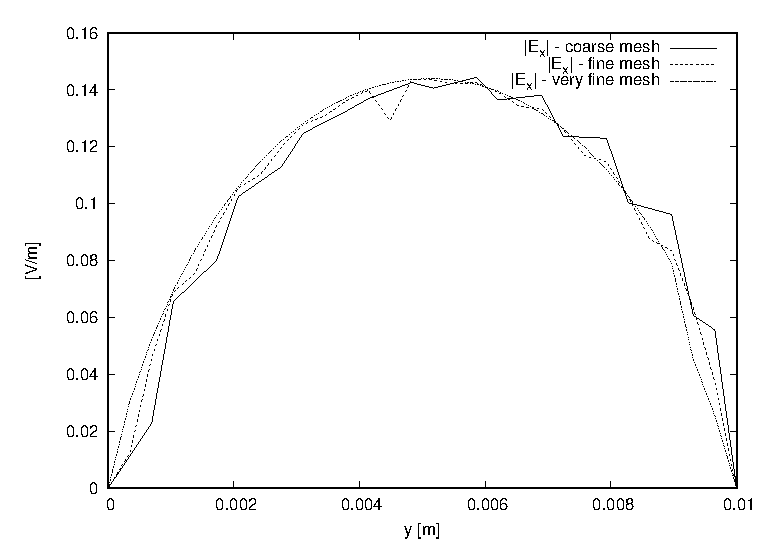
\includegraphics{figure_convergence_alotto_codecasa_along_y_mag_ex.eps}
\caption{Convergence of the solution for problem involving medium in \cite{alottocodecasa}.
The magnitude of the $x$ component of the electric field is plotted
along a line parallel to $y$ axis for four different meshes.}
\label{fi:alotto_codecasa_convergence}
\end{figure}

We provide the magnitudes and phases of the components of the electric field obtained from the 
simulation in Figures \ref{fi:alotto_codecasa_xaxis_ex} to \ref{fi:alotto_codecasa_zaxis_ez}.
It can be observed that the bianisotropic effects are non negligible and the largest effects 
are on the x component of the field.
The bianisotropy causes a difference in magnitude of up to 14 percent of the incident 
field, as can be seen,  for example, from Figure  \ref{fi:alotto_codecasa_xaxis_ex}, 
\ref{fi:alotto_codecasa_yaxis_ex} or  \ref{fi:alotto_codecasa_zaxis_ex}.
Since the theory guarantees the reliability of these results, it can be used as benchmark for 
other solvers and approaches.


\begin{figure}
\centering
\begin{subfigure}[b]{0.49\textwidth}
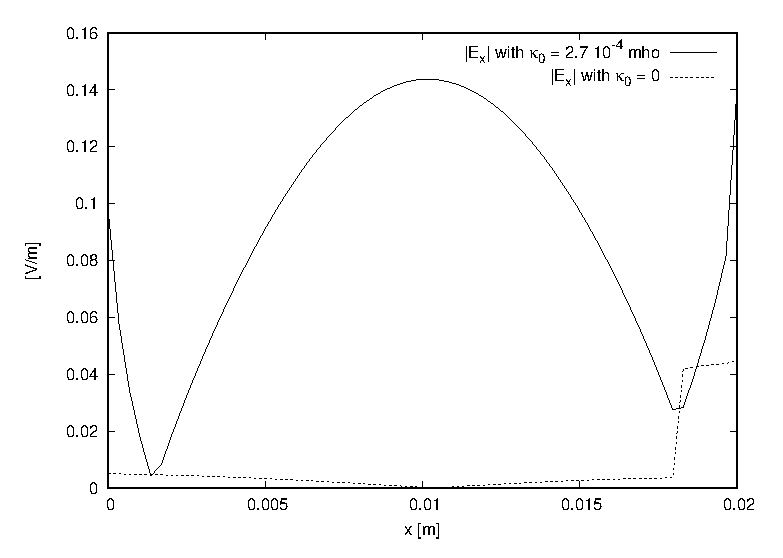
\includegraphics[width=\textwidth]{figure_alotto_codecasa_along_x_mag_ex.eps}
\end{subfigure}
%
\begin{subfigure}[b]{0.49\textwidth}
\centering
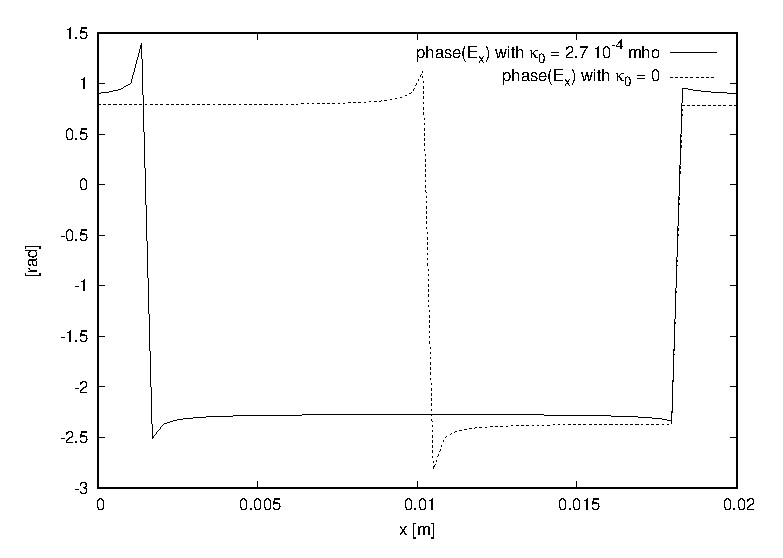
\includegraphics[width=\textwidth]{figure_alotto_codecasa_along_x_phase_ex.eps}
\end{subfigure}
\caption{The magnitude and phase of the $x$ component of electric field along a line parallel to $x$ axis 
and passing though the center of gravity of the domain for problem involving 
medium in \cite{alottocodecasa}. 
The plot for bianisotropic case  using $\kappa_0 = 2.7\,10^{-4}$ mho is compared with 
the solution obtained in isotropic case using $\kappa_0 = 0$.}
\label{fi:alotto_codecasa_xaxis_ex}
\end{figure}

\begin{figure}
\centering
\begin{subfigure}[b]{0.49\textwidth}
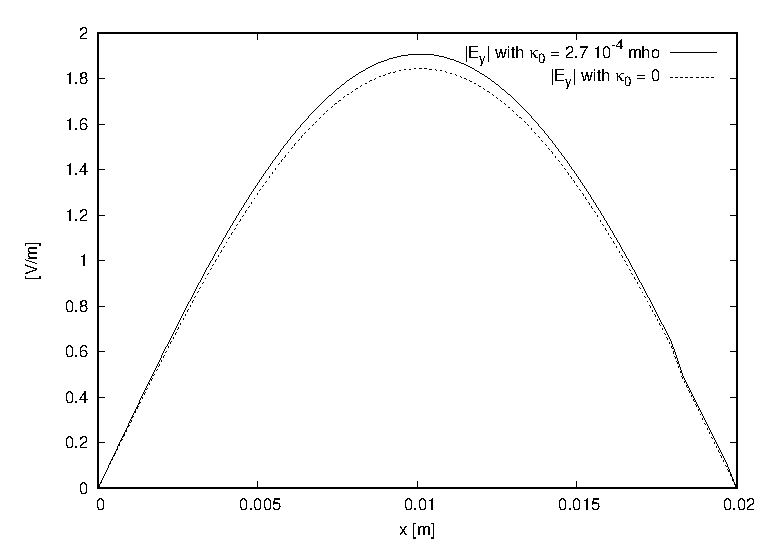
\includegraphics[width=\textwidth]{figure_alotto_codecasa_along_x_mag_ey.eps}
\end{subfigure}
%
\begin{subfigure}[b]{0.49\textwidth}
\centering
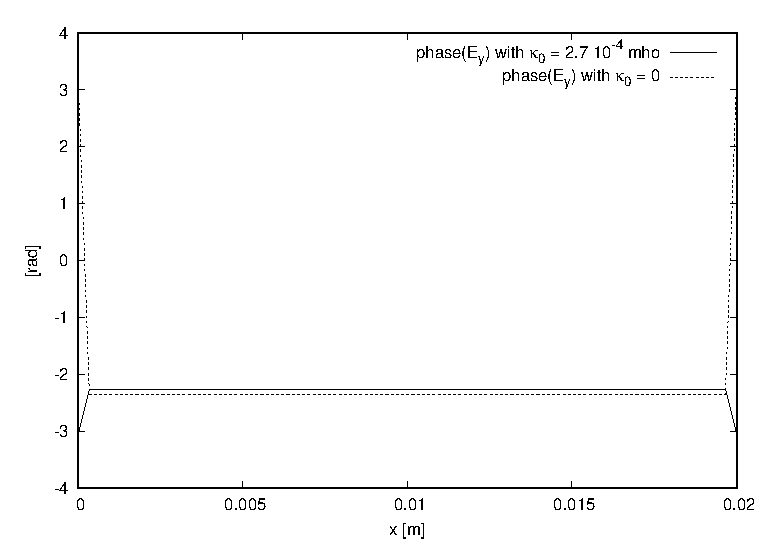
\includegraphics[width=\textwidth]{figure_alotto_codecasa_along_x_phase_ey.eps}
\end{subfigure}
\caption{The magnitude and phase of the $y$ component of electric field along a line parallel to $x$ axis 
and passing though the center of gravity of the domain for problem involving 
medium in \cite{alottocodecasa}. 
The plot for bianisotropic case  using $\kappa_0 = 2.7\,10^{-4}$ mho is compared with 
the solution obtained in isotropic case using $\kappa_0 = 0$.}
\label{fi:alotto_codecasa_xaxis_ey}
\end{figure}

\begin{figure}
\centering
\begin{subfigure}[b]{0.49\textwidth}
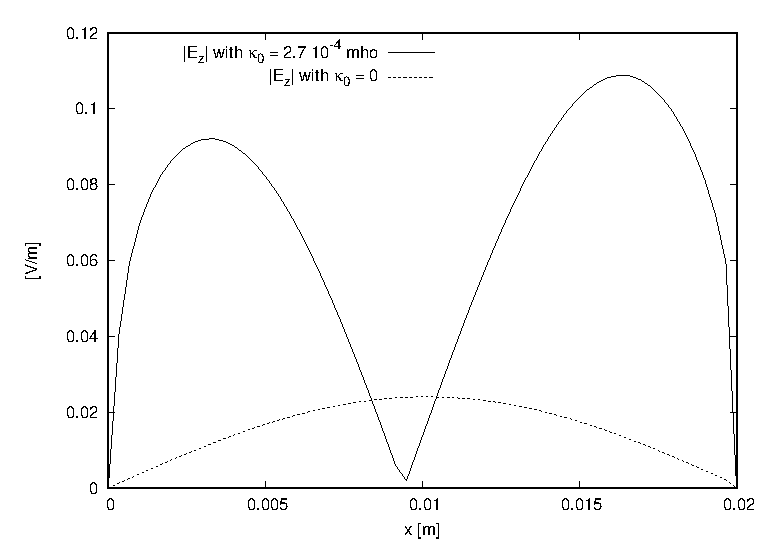
\includegraphics[width=\textwidth]{figure_alotto_codecasa_along_x_mag_ez.eps}
\end{subfigure}
%
\begin{subfigure}[b]{0.49\textwidth}
\centering
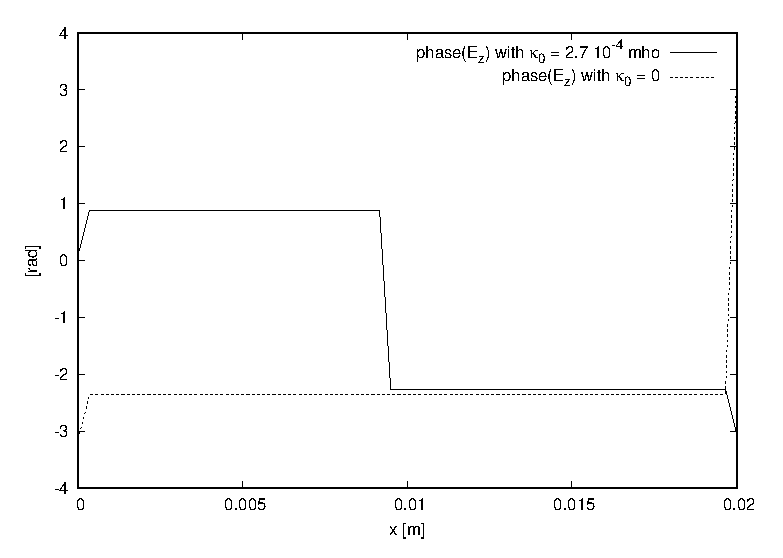
\includegraphics[width=\textwidth]{figure_alotto_codecasa_along_x_phase_ez.eps}
\end{subfigure}
\caption{The magnitude and phase of the $z$ component of electric field along a line parallel to $x$ axis 
and passing though the center of gravity of the domain for problem involving 
medium in \cite{alottocodecasa}. 
The plot for bianisotropic case  using $\kappa_0 = 2.7\,10^{-4}$ mho is compared with 
the solution obtained in isotropic case using $\kappa_0 = 0$.}
\label{fi:alotto_codecasa_xaxis_ez}
\end{figure}

\begin{figure}
\centering
\begin{subfigure}[b]{0.49\textwidth}
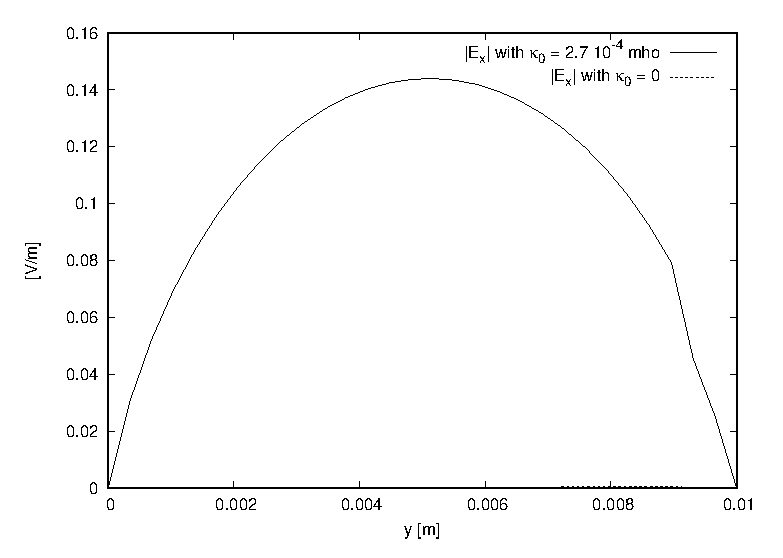
\includegraphics[width=\textwidth]{figure_alotto_codecasa_along_y_mag_ex.eps}
\end{subfigure}
%
\begin{subfigure}[b]{0.49\textwidth}
\centering
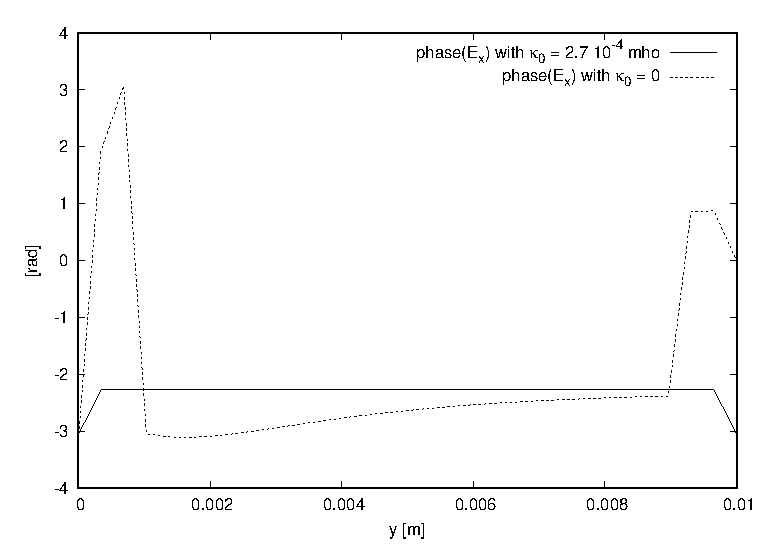
\includegraphics[width=\textwidth]{figure_alotto_codecasa_along_y_phase_ex.eps}
\end{subfigure}
\caption{The magnitude and phase of the $x$ component of electric field along a line parallel to $y$ axis 
and passing though the center of gravity of the domain for problem involving 
medium in \cite{alottocodecasa}. 
The plot for bianisotropic case  using $\kappa_0 = 2.7\,10^{-4}$ mho is compared with 
the solution obtained in isotropic case using $\kappa_0 = 0$.}
\label{fi:alotto_codecasa_yaxis_ex}
\end{figure}

\begin{figure}
\centering
\begin{subfigure}[b]{0.49\textwidth}
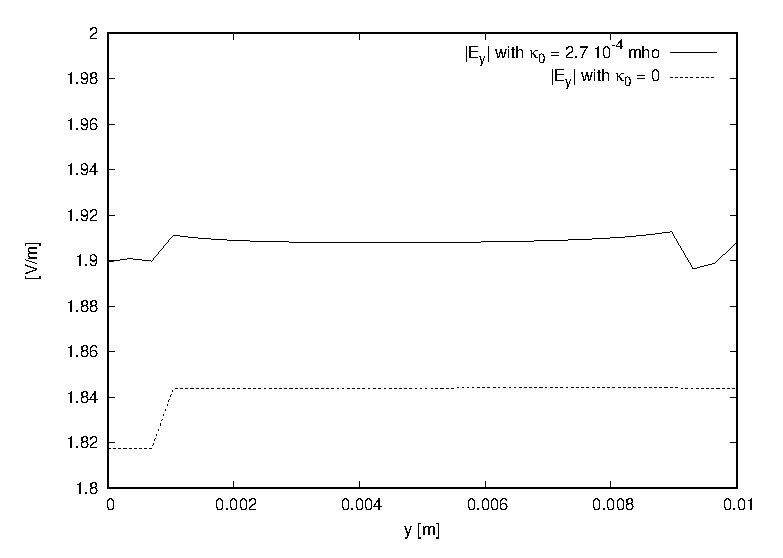
\includegraphics[width=\textwidth]{figure_alotto_codecasa_along_y_mag_ey.eps}
\end{subfigure}
%
\begin{subfigure}[b]{0.49\textwidth}
\centering
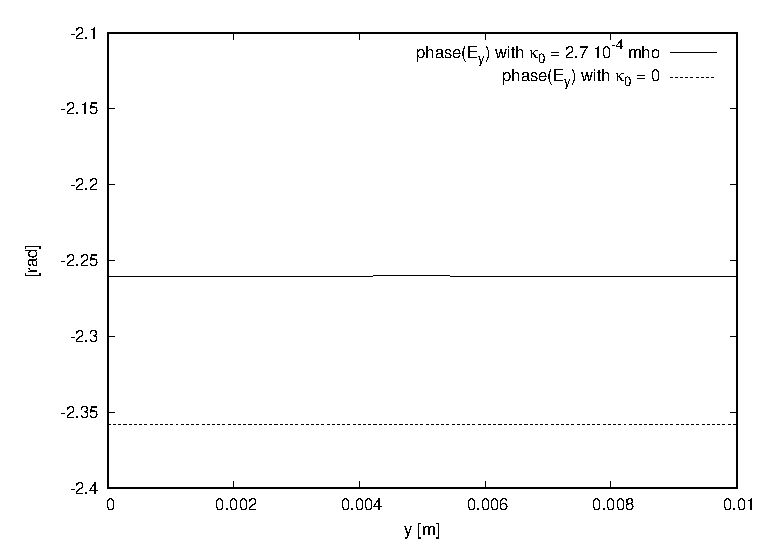
\includegraphics[width=\textwidth]{figure_alotto_codecasa_along_y_phase_ey.eps}
\end{subfigure}
\caption{The magnitude and phase of the $y$ component of electric field along a line parallel to $y$ axis 
and passing though the center of gravity of the domain for problem involving 
medium in \cite{alottocodecasa}. 
The plot for bianisotropic case  using $\kappa_0 = 2.7\,10^{-4}$ mho is compared with 
the solution obtained in isotropic case using $\kappa_0 = 0$.}
\label{fi:alotto_codecasa_yaxis_ey}
\end{figure}

\begin{figure}
\centering
\begin{subfigure}[b]{0.49\textwidth}
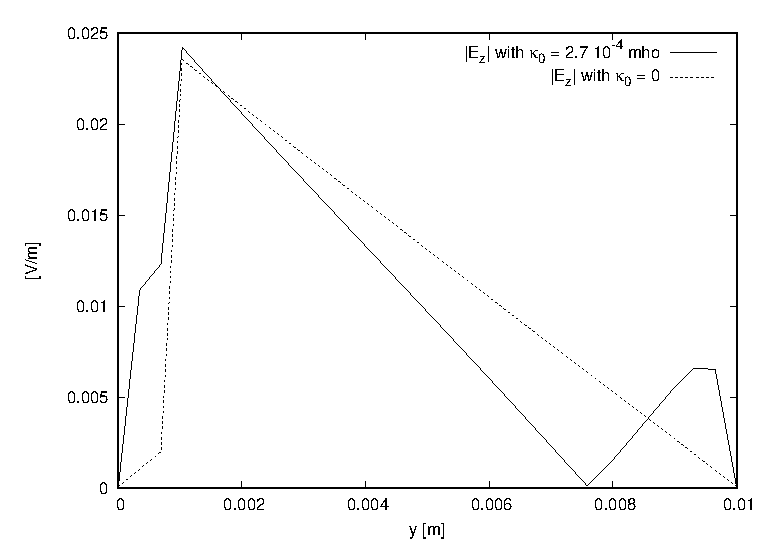
\includegraphics[width=\textwidth]{figure_alotto_codecasa_along_y_mag_ez.eps}
\end{subfigure}
%
\begin{subfigure}[b]{0.49\textwidth}
\centering
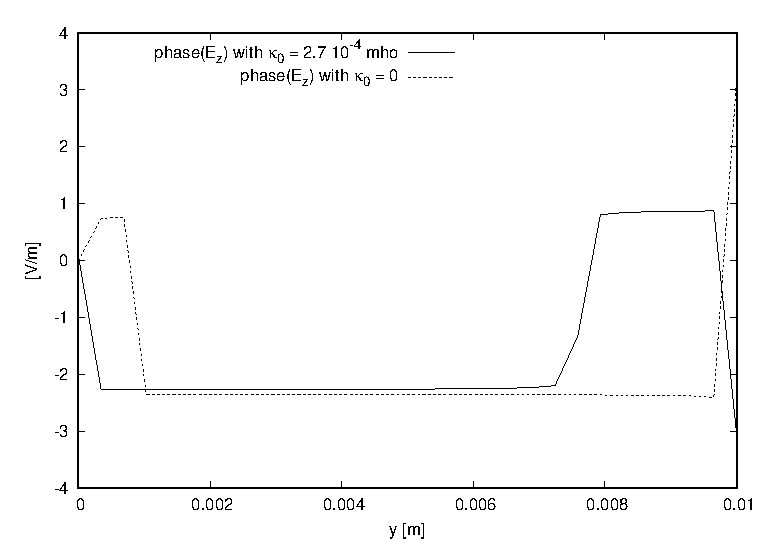
\includegraphics[width=\textwidth]{figure_alotto_codecasa_along_y_phase_ez.eps}
\end{subfigure}
\caption{The magnitude and phase of the $z$ component of electric field along a line parallel to $y$ axis 
and passing though the center of gravity of the domain for problem involving 
medium in \cite{alottocodecasa}. 
The plot for bianisotropic case  using $\kappa_0 = 2.7\,10^{-4}$ mho is compared with 
the solution obtained in isotropic case using $\kappa_0 = 0$.}
\label{fi:alotto_codecasa_yaxis_ez}
\end{figure}

\begin{figure}
\centering
\begin{subfigure}[b]{0.49\textwidth}
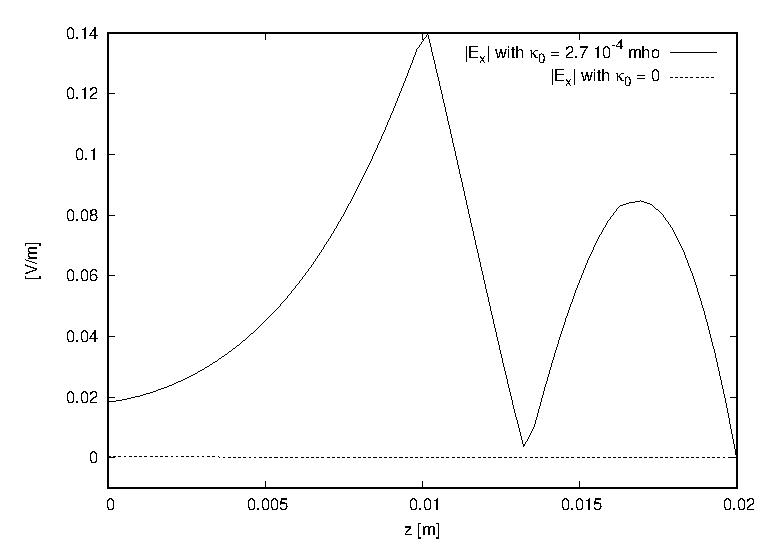
\includegraphics[width=\textwidth]{figure_alotto_codecasa_along_z_mag_ex.eps}
\end{subfigure}
%
\begin{subfigure}[b]{0.49\textwidth}
\centering
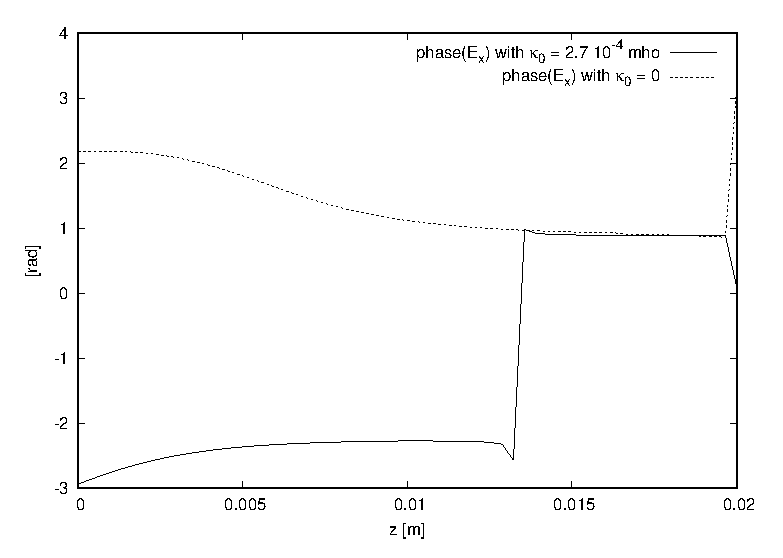
\includegraphics[width=\textwidth]{figure_alotto_codecasa_along_z_phase_ex.eps}
\end{subfigure}
\caption{The magnitude and phase of the $x$ component of electric field along a line parallel to $z$ axis 
and passing though the center of gravity of the domain for problem involving 
medium in \cite{alottocodecasa}. 
The plot for bianisotropic case  using $\kappa_0 = 2.7\,10^{-4}$ mho is compared with 
the solution obtained in isotropic case using $\kappa_0 = 0$.}
\label{fi:alotto_codecasa_zaxis_ex}
\end{figure}

\begin{figure}
\centering
\begin{subfigure}[b]{0.49\textwidth}
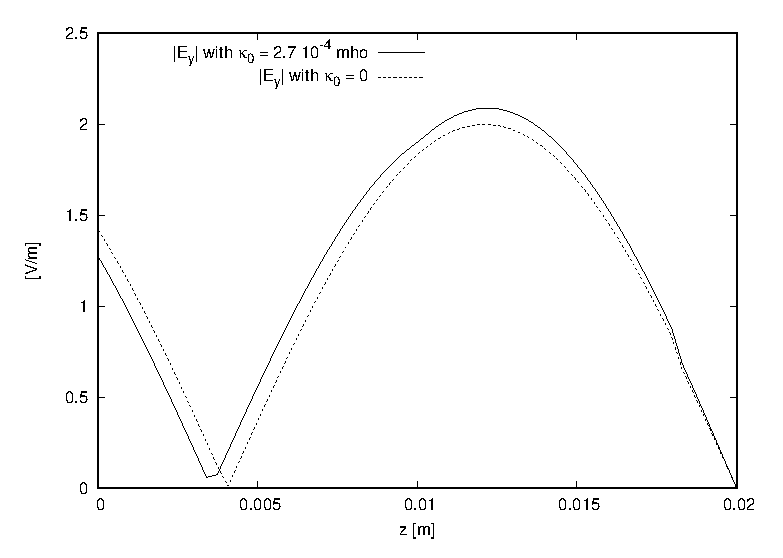
\includegraphics[width=\textwidth]{figure_alotto_codecasa_along_z_mag_ey.eps}
\end{subfigure}
%
\begin{subfigure}[b]{0.49\textwidth}
\centering
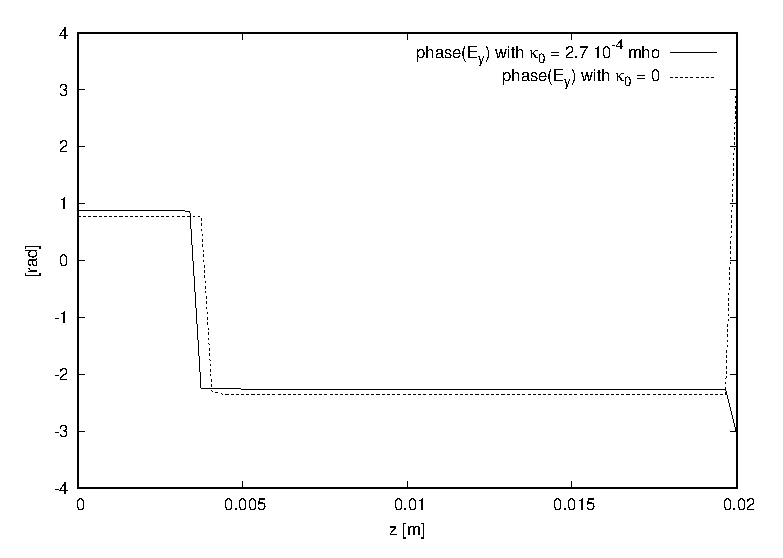
\includegraphics[width=\textwidth]{figure_alotto_codecasa_along_z_phase_ey.eps}
\end{subfigure}
\caption{The magnitude and phase of the $y$ component of electric field along a line parallel to $z$ axis 
and passing though the center of gravity of the domain for problem involving 
medium in \cite{alottocodecasa}. 
The plot for bianisotropic case  using $\kappa_0 = 2.7\,10^{-4}$ mho is compared with 
the solution obtained in isotropic case using $\kappa_0 = 0$.}
\label{fi:alotto_codecasa_zaxis_ey}
\end{figure}

\begin{figure}
\centering
\begin{subfigure}[b]{0.49\textwidth}
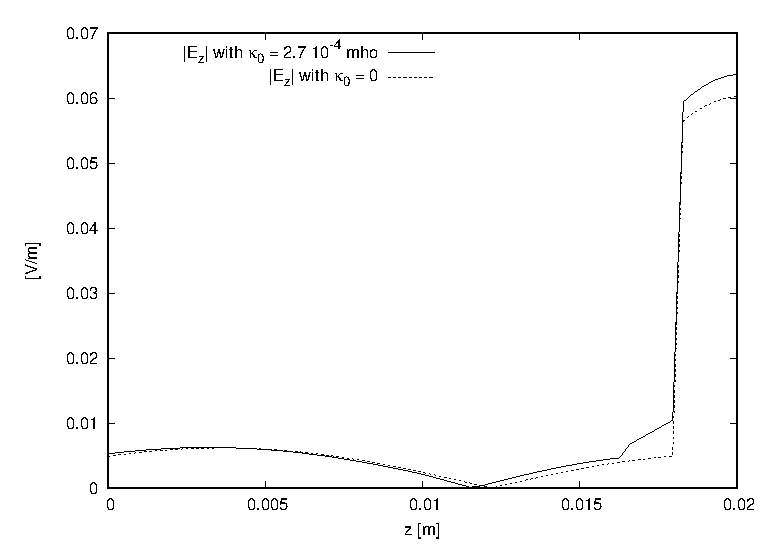
\includegraphics[width=\textwidth]{figure_alotto_codecasa_along_z_mag_ez.eps}
\end{subfigure}
%
\begin{subfigure}[b]{0.49\textwidth}
\centering
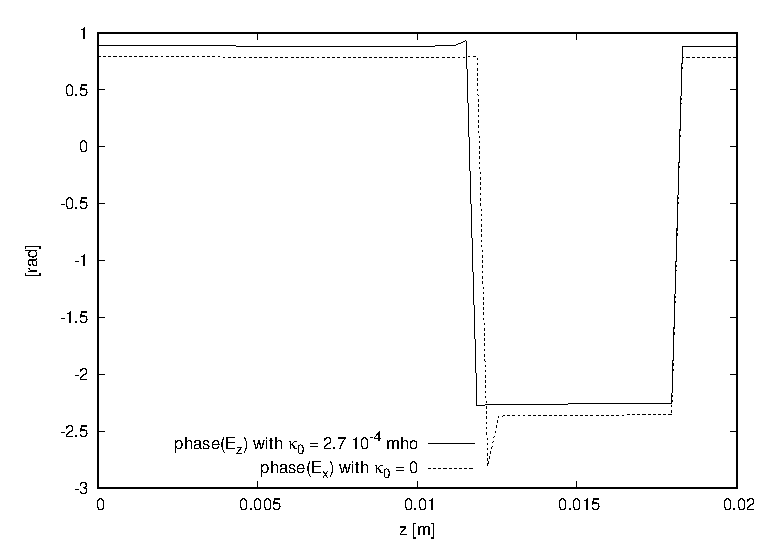
\includegraphics[width=\textwidth]{figure_alotto_codecasa_along_z_phase_ez.eps}
\end{subfigure}
\caption{The magnitude and phase of the $z$ component of electric field along a line parallel to $z$ axis 
and passing though the center of gravity of the domain for problem involving 
medium in \cite{alottocodecasa}. 
The plot for bianisotropic case  using $\kappa_0 = 2.7\,10^{-4}$ mho is compared with 
the solution obtained in isotropic case using $\kappa_0 = 0$.}
\label{fi:alotto_codecasa_zaxis_ez}
\end{figure}
